% Template for ICIP-2022 paper; to be used with:
%          spconf.sty  - ICASSP/ICIP LaTeX style file, and
%          IEEEbib.bst - IEEE bibliography style file.
% --------------------------------------------------------------------------
\documentclass{article}
\usepackage{spconf,amsmath,graphicx, booktabs, array, subfig}
\usepackage{amssymb}% http://ctan.org/pkg/amssymb
\usepackage{pifont}% http://ctan.org/pkg/pifont
\usepackage{xcolor}
\usepackage[colorlinks,allcolors=blue]{hyperref}
\usepackage{verbatim}

\newcommand{\chmark}{\ding{51}}
\newcommand{\crmark}{\ding{55}}
\newcommand{\source}[1]{\texttt{#1}}
\newcommand{\alex}[1]{{\color{blue} A: #1}}
\newcommand{\simon}[1]{{\color{red} S: #1}}


% Example definitions.
% --------------------
\def\x{{\mathbf x}}
\def\L{{\cal L}}

% Title.
% ------
% \title{A NEW ARCHITECTURE FOR MUSIC SOURCE SEPARATION: HYBRID TRANSFORMER DEMUCS}
\title{hybrid transformers for music source separation}
%
% Single address.
% ---------------
\name{Simon Rouard, Francisco Massa, Alexandre D{\'{e}}fossez}
\address{Meta AI}
%
% For example:
% ------------
%\address{School\\
%	Department\\
%	Address}
%
% Two addresses (uncomment and modify for two-address case).
% ----------------------------------------------------------
%\twoauthors
%  {A. Author-one, B. Author-two\sthanks{Thanks to XYZ agency for funding.}}
%	{School A-B\\
%	Department A-B\\
%	Address A-B}
%  {C. Author-three, D. Author-four\sthanks{The fourth author performed the work
%	while at ...}}
%	{School C-D\\
%	Department C-D\\
%	Address C-D}
%
\begin{document}
%\ninept
%
\maketitle
%
\begin{abstract}
% The latest advances in Music source Separation (MSS) has seen strong gains by using deep learning based models.
A natural question arising in Music Source Separation (MSS) is whether long range contextual information is useful,
or whether local acoustic features are sufficient.
In other fields, attention based Transformers~\cite{transformer} have shown their ability to integrate
information over long sequences. In this work, we introduce Hybrid Transformer Demucs (HT Demucs), 
an hybrid temporal/spectral bi-U-Net based on Hybrid Demucs~\cite{defossez2021hybrid}, 
where the innermost layers are replaced by a cross-domain Transformer Encoder, 
using self-attention within one domain, and cross-attention across domains.
While it performs poorly when trained only on MUSDB~\cite{musdb}, we show that it outperforms Hybrid Demucs (trained on the same data) by 0.45 dB of SDR when using 800 extra training songs.
Using sparse attention kernels to extend its receptive field, and per source fine-tuning, 
we achieve state-of-the-art results on MUSDB with extra training data, with 9.20 dB of SDR.

% The latest advances in Music Source Separation (MSS) use deep learning models that mix spectrogram and waveform domains such as Hybrid Demucs \cite{defossez2021hybrid} or KUIELAB-MDX-Net \cite{kuielab}. In this work, we present a novel deep learning architecture for Music Source Separation (MSS) named Hybrid Transformer Demucs.
% This new architecture is based on Hybrid Demucs with architectural simplifications and the addition of a Cross Transformer Encoder that alternatively computes self-attention and cross-attention within and between each domain. This Transformer is located after the last downsampling layers of the U-Nets in order to process compact sequences. By training on the MUSDB18HQ dataset \cite{musdb18-hq} combined with 800 more songs, our best model achieves an SDR of ???. 
\end{abstract}
%
\begin{keywords}
Music Source Separation, Transformers
\end{keywords}
%
\section{Introduction}
\label{sec:intro}

Since the 2015 Signal Separation Evaluation Campaign (SiSEC) \cite{sisec15}, the community of MSS has mostly focused on the task of training supervised models to separate songs into 4 stems: drums, bass, vocals and other (all the other instruments). The reference dataset that is used to benchmark MSS is MUSDB18~\cite{musdb,musdb18-hq} which is made of 150 songs in two versions (HQ and non-HQ). 
Its training set is composed of 87 songs, a relatively small corpus compared with other deep learning based tasks, where Transformer~\cite{transformer} based architectures have seen widespread success and adoption, such as vision~\cite{layerscale,Rombach_2022_CVPR} or natural language tasks~\cite{brown2020language}. Source separation is a task where having a short context or a long context as input both make sense. Conv-Tasnet~\cite{convtasnet} uses about one second of context to perform the separation, using only local acoustic features. On the other hand, Demucs~\cite{demucsv2} can use up to 10 seconds of context, which can help to resolve ambiguities in the input. In the present work, we aim at studying how Transformer architectures can help leverage this context, and what amount of data is required to train them.

We first present in Section~\ref{sec:architecture} a novel architecture, \emph{Hybrid Transformer Demucs} (HT Demucs), which replaces the innermost layers of the original Hybrid Demucs architecture~\cite{defossez2021hybrid} with Transformer layers, applied both in the time and spectral
representation, using self-attention within one domain, and cross-attention across domains.
% While the original bi-U-net structure required careful design of the strides and padding to align the two representations,
% the attention mechanism removes the need for manual alignment. 
As Transformers are usually data hungry, we leverage an internal dataset composed of 800 songs on top of the MUSDB dataset, described in Section~\ref{sec:dataset}. 

Our second contribution is to evaluate extensively this new architecture in Section~\ref{sec:results}, with various settings (depth, number of channels, context length, augmentations etc.). We show in particular that it improves over the baseline Hybrid Demucs architecture (retrained on the same data) by 0.35~dB. 

Finally, we experiment with increasing the context duration using sparse kernels based with Locally Sensitive Hashing
to overcome memory issues during training, and fine-tuning procedure, thus achieving a final SDR of 9.20~dB on the test set of MUSDB. 

We release the training code, pre-trained models, and samples on our github~\href{https://github.com/facebookresearch/demucs}{facebookresearch/demucs.}



% However, since we want the best performing models, lots of related work use extra data. In our case, we currated an internal dataset and kept 800 songs for the training set.
% In Tab.~\ref{tab:baselines}, we display the results of our best model compared to other models that have been trained on MUSDB18 and extra data. These models are Hybrid Demucs \cite{defossez2021hybrid} and KUIELAB-MDX-Net which are hybrid architectures that operate both in the spectral and waveform domain, Band-Split RNN \cite{bsrnn} is a frequency-domain model that splits the spectrogram of the mixture into subbands and perform interleaved band-level and sequence-level modeling with RNNs, Demucs v2 \cite{demucsv2} is the ancestor of Hybrid Demucs working in the waveform domain, D3Net \cite{d3net} is a dilated convolutional network working in the frequency domain and Spleeter \cite{spleeter} is based on a U-Net architecture in the frequency domain \cite{unet} and uses a large extra dataset. Notice that the results of Hybrid Demucs that we provide are based on this dataset. In addition, we couldn't report the results of KUIELAB-MDX-Net on a large dataset since the authors used the test set of MUSDB18 in their extra training set for the 2021 Music Demixing Challenge \cite{mdx2021}. We also provide the metrics for the Ideal Ratio Mask oracle (IRM) \cite{sisec18}, which computes the best possible mask using the ground truth sources. The IRM oracle sets a higher band for spectrogram masking based models. On our dataset, Hybrid Transformer Demucs outperforms Hybrid Demucs by almost +??(0.7 dB).

\section{Related Work}
\label{sec:related}

% \alex{add missing baselines: spleeter, ResUNetDecouple+, CWS-PResUNet maybe ?}
% \simon{I added an explanation for spleeter, but ResUNetDecouple+, CWS-PResUNet are quite bad on bass drums and other so I dont know if we should add them?}
A traditional split for MSS methods is between spectrogram based and waveform based models.
The former includes models like Open-Unmix~\cite{umx}, a biLSTM with fully connected that
predicts a mask on the input spectrogram or D3Net~\cite{d3net} which uses dilated convolutional blocks with dense connections. More recently, using complex-spectrogram as input and output was favored~\cite{lasaft} as it provides a richer representation and removes the topline given by the Ideal-Ratio-Mask.
The latest spectrogram model, Band-Split RNN~\cite{bsrnn}, combines this idea, along with multiple
dual-path RNNs~\cite{luo2020dual}, each acting in carefully crafted frequency band. 
It currently achieves the state-of-the-art on MUSDB with 8.9 dB.
Waveform based models started with Wave-U-Net~\cite{waveunet}, which served as the basis for Demucs~\cite{demucsv2}, a 
time domain U-Net with a bi-LSTM between the encoder and decoder. Around the same time, Conv-TasNet
showed competitive results~\cite{convtasnet,demucsv2} using residual dilated convolution blocks to predict
a mask over a learnt representation. Finally, a recent trend has been to use both temporal and spectral domains, either through model blending, like KUIELAB-MDX-Net~\cite{kuielab}, or using
a bi-U-Net structure with a shared backbone as Hybrid Demucs~\cite{defossez2021hybrid}. Hybrid Demucs
was the first ranked architecture at the latest MDX MSS Competition~\cite{mdx2021}, although
it is now surpassed by Band-Split RNN.

Using large datasets has been shown to be beneficial to the task of MSS.
Spleeter \cite{spleeter} is a spectrogram masking U-Net architecture trained on 25,000 songs extracts of 30 seconds,
and was at the time of its release, the best model available. Both D3Net and Demucs highly benefited from
using extra training data, while still offering strong performance on MUSDB only.
Band-Split RNN introduced a novel unsupervised augmentation technique requiring only mixes to improve its 
performance by 0.7 dB of SDR.

Transformers have been used for speech source separation with SepFormer~\cite{subakan2021attention},  which is similar to Dual-Path RNN: short range attention layers are interleaved with long range ones.
However, its requires almost 11GB of memory for the forward pass for 5 seconds of audio at 8 kHz, and thus is not 
adequate for studying longer inputs at 44.1 kHz.
% Our early experiments
% did not show any gain by using this instead of regular Transformers. 
% The difference could be explained by the low sample rate used to train it for
% speech source separation (8kHz).
% \alex{todo add
% some motivation, why not use sepformer, e.g. compute receptive field maybe, also originally in 8kHz,
% plus our early experiments.} \simon{done}



\begin{table}
\caption{Comparison with baselines on the test set of MUSDB HQ (methods with a $^*$ are reported on the non HQ version). ``Extra?'' indicates the number of 
extra songs used at train time, $\dagger$ indicates that only mixes are used. ``fine tuned'' indices
per source fine-tuning.}
\label{tab:baselines}
\begin{center}
%   \setlength\extrarowheight{2pt}
\resizebox{0.48\textwidth}{!}{
\begin{tabular}{l c r r r r r}
  \toprule
     &&& \multicolumn{4}{c}{Test SDR in dB}\\
     \cmidrule{3-7}
  \textbf{Architecture} & \textbf{Extra?} &
  \source{All} & \source{Drums} &  \source{Bass} &\source{Other} & \source{Vocals}\\
  \midrule
  IRM oracle & N/A & 8.22 & 8.45 & 7.12 & 7.85 & 9.43\\
  \midrule
  KUIELAB-MDX-Net \cite{kuielab} & \crmark & 7.54 &7.33&7.86&5.95& 9.00 \\
  Hybrid Demucs \cite{defossez2021hybrid} & \crmark & 7.64 & 8.12 & 8.43 & 5.65 & 8.35 \\
  Band-Split RNN \cite{bsrnn} & \crmark & \textbf{8.24} & 9.01 & 7.22 & 6.70 & 10.01 \\
  \midrule
  HT Demucs & \crmark & 7.52 & 7.94 & 8.48 & 5.72 & 7.93  \\
  \midrule
  Spleeter$^*$ \cite{spleeter} & $25\mathrm{k}$ & 5.91 & 6.71 & 5.51 & 4.55 & 6.86\\
  D3Net$^*$ \cite{d3net} & 1.5k & 6.68 & 7.36  & 6.20 & 5.37 & 7.80 \\
  Demucs v2$^*$ \cite{demucsv2} & 150 & 6.79 & 7.58 & 7.60 & 4.69 & 7.29  \\
  Hybrid Demucs \cite{defossez2021hybrid} & 800 & 8.34 &9.31&9.13& 6.18& 8.75  \\
  Band-Split RNN \cite{bsrnn} & 1750$^\dagger$ & 8.97 & 10.15 & 8.16 & \textbf{7.08} & \textbf{10.47} \\
  \midrule
  HT Demucs & 150 & 8.49 & 9.51 & 9.76 & 6.13 & 8.56  \\
  HT Demucs & 800 & 8.80 & 10.05 & 9.78 & 6.42 & 8.93  \\
  HT Demucs (fine tuned) & 800 & 9.00 & 10.08 & 10.39 & 6.32 & 9.20  \\
  Sparse HT Demucs (fine tuned) & 800 & \textbf{9.20} & \textbf{10.83} & \textbf{10.47} & 6.41 & 9.37  \\
  \bottomrule
\end{tabular}}
\end{center}
\vspace{-0.1cm}
{\footnotesize }
\end{table}


\section{Architecture}
\label{sec:architecture}

\begin{figure*}[h]
    \centering
    \subfloat[\centering Transformer Encoder Layer]{{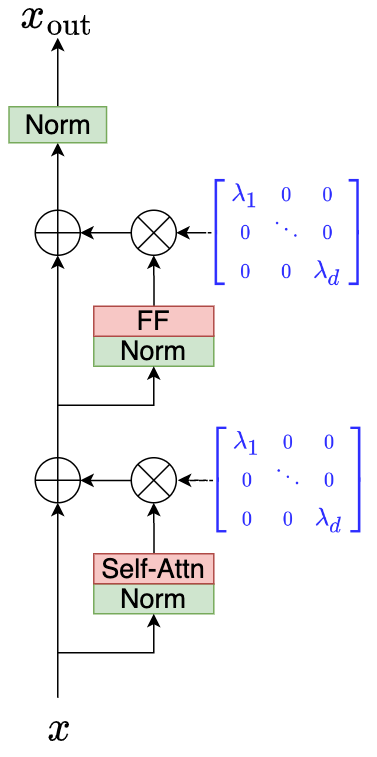
\includegraphics[width=2.6cm]{imgs/encoder_.png} }}%
    \qquad
    \subfloat[\centering Cross-domain Transformer Encoder of depth 5]{{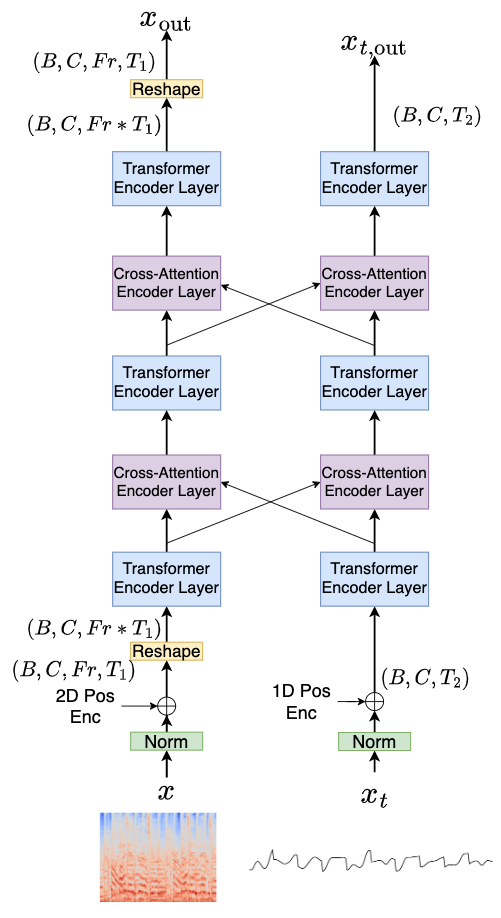
\includegraphics[width=5cm]{imgs/transformer_.png} }}%
    \qquad
    \subfloat[\centering Hybrid Transformer Demucs]{{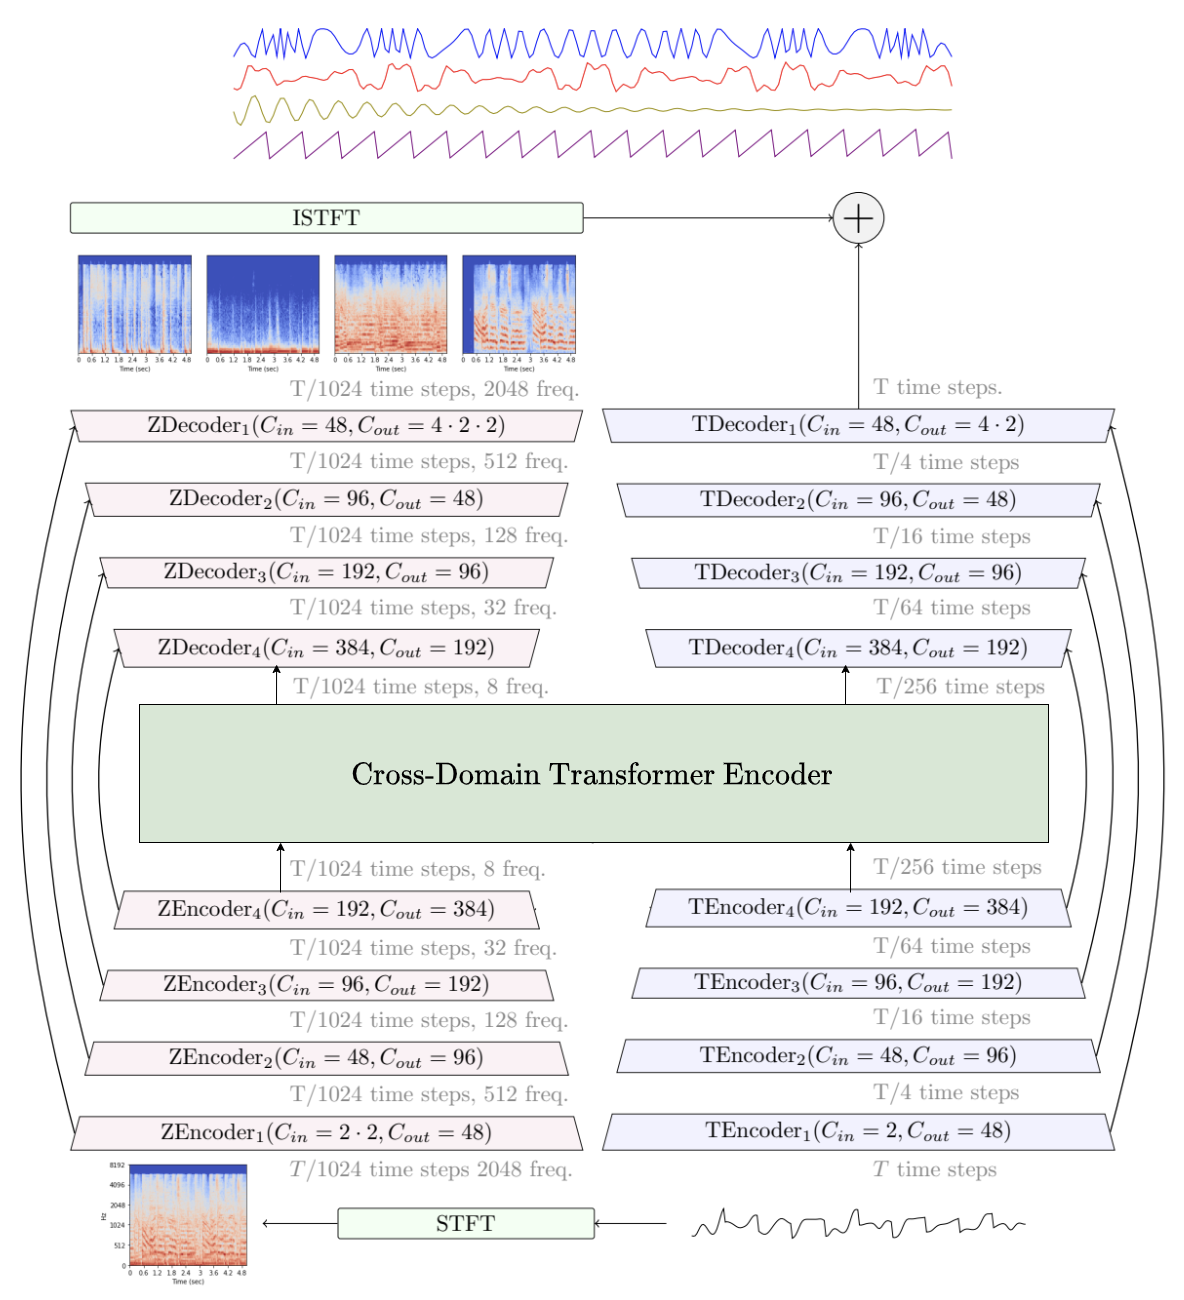
\includegraphics[width=8.5cm]{imgs/htdemucs__.png} }}%
    \caption{Details of the Hybrid Transformer Demucs architecture. (a): the Transformer Encoder layer
        with self-attention and Layer Scale \cite{layerscale}. (b): The Cross-domain Transformer Encoder treats spectral and temporal signals with interleaved Transformer Encoder layers and cross-attention Encoder layers. (c): Hybrid Transformer Demucs keeps the outermost 4 encoder and decoder layers of Hybrid Demucs with the addition of a cross-domain Transformer Encoder between them.}
    \label{fig:architecture}%
\end{figure*}

We introduce the Hybrid Transformer Demucs model, based on Hybrid Demucs~\cite{defossez2021hybrid}.
The original Hybrid Demucs model is made of two U-Nets, one in the time domain (with temporal convolutions) and
one in the spectrogram domain (with convolutions over the frequency axis). 
Each U-Net is made of 5 encoder layers, and 5 decoder layers. After the 5-th encoder layer, both representation
have the same shape, and they are summed before going into a shared 6-th layer. Similarly, the first decoder layer is shared, and
its output is sent both the temporal and spectral branch. The output of the spectral branch
is transformed to a waveform using the iSTFT, before being summed with the output of the temporal branch, giving the 
actual prediction of the model.

Hybrid Transformer Demucs keeps the outermost 4 layers as is from the original architecture, and replaces the 2 innermost layers in the encoder and the decoder, including local attention and bi-LSTM, with
a cross-domain Transformer Encoder.
It treats in parallel the 2D signal from the spectral branch and the 1D signal from the waveform branch. 
Unlike the original Hybrid Demucs which required careful tuning of the model parameters (STFT window and hop length, stride, paddding, etc.) to align the time and spectral representation, the cross-domain
Transformer Encoder can work with heterogeneous data shape, making it a more flexible architecture.

% Hybrid Demucs needs very specific parameters for the STFT and the number of channels of the encoder blocks in order to have a flat spectral representation (i.e. no frequency dimension) after the 5th encoder block so that it can be summed with the downsampled temporal representation. Moreover, the compressed residual branchs of the encoder use custom Local Attention and Bi-LSTM modules for the 5th and 6th blocks. \\
The architecture of Hybrid Transformer Demucs is depicted on Fig.\ref{fig:architecture}. On the left, we show a single self-attention Encoder layer of the Transformer~\cite{transformer} with normalizations before the Self-Attention and Feed-Forward operations, it is combined with Layer Scale \cite{layerscale} initialized to $\epsilon{=}10^{-4}$ in order to stabilize the training. The two first normalizations are layer normalizations (each token is independently normalized) and the third one is a time layer normalization (all the tokens are normalized together). 
The input/output dimension of the Transformer is $384$, and linear layers are used to convert to the internal
dimension of the Transformer when required.
The attention mechanism has 8 heads and the hidden state size of the feed forward network is equal to 4 times the dimension of the transformer. The cross-attention Encoder layer is the same but using cross-attention with the other domain representation. In the middle, a cross-domain Transformer Encoder of depth 5 is depicted. It is the interleaving of self-attention Encoder layers and cross-attention Encoder layers in the spectral and waveform domain. 1D \cite{transformer} and 2D \cite{2Dpe} sinusoidal encodings are added to the scaled inputs and reshaping is applied to the spectral representation in order to treat it as a sequence. On Fig.~\ref{fig:architecture} (c), we give
a representation of the entire architecture, along with the double U-Net encoder/decoder structure.

Memory consumption and the speed of attention quickly deteriorates with an increase of the sequence lengths.
To further scale, we leverage sparse attention kernels introduced in the \texttt{xformer} package~\cite{xFormers2021},
along with a Locally Sensitive Hashing (LSH) scheme to determine dynamically the sparsity pattern. We use a sparsity level
of 90\% (defined as the proportion of elements removed in the softmax), which is determined by performing 32 rounds of LSH with 4 buckets each. We select the elements that match at least $k$ times over all 32 rounds of LSH, with $k$ such that the sparsity level is 90\%.
% by a random projection to a 32 dimension space, with 4 random separating hyperplans.
We refer to this variant as Sparse HT Demucs.


\section{Dataset}
\label{sec:dataset}
We curated an internal dataset composed of 3500 songs with the stems from 200 artists with diverse music genres. Each stem is assigned to one of the 4 sources according to the name given by the music producer (for instance "vocals2", "fx", "sub" etc...). This labeling is noisy because these names are subjective and sometime ambiguous. 
For 150 of those tracks, we manually verified that the automated 
labeling was correct, and discarded ambiguous stems. 
We trained a first Hybrid Demucs model on MUSDB and those 150 tracks.
We preprocess the dataset according to several rules.
First, we keep only the stems for which all four sources are non silent at least 30\% of the time. For each 1 second segment, we define it as silent if its volume is less than -40dB. 
% First, we gathered the labels \textit{percussion and drums} into \textit{drums}, we gathered \textit{guitar, keyboard, piano, brass, woodwind, string, synth} into \textit{other} and we kept the classes \textit{vocals} and \textit{bass}. 
Second, for a song $x$ of our dataset, noting $x_i$, with $i \in \{\mathrm{drums, bass, other, vocals} \}$, each stem and $f$ the Hybrid Demucs model previously mentioned, we define $y_{i,j}{=}f(x_i)_j$ i.e. the output $j$ when separating the stem $i$. Theoretically, if all the stems were perfectly labeled and if $f$ were a perfect source separation model we would have $y_{i, j} = x_i \delta_{i, j}$ with $\delta_{i, j}$ being the Kronecker delta.
For a waveform $z$, let us define the volume in dB measured over 1 second segments:
\begin{equation}
    V(z) = 10\cdot\log_{10}\left(\mathrm{AveragePool}(z^2, 1\text{ sec})\right).
\end{equation}
For each pair of sources $i,j$, we take the segments of 1 second where the stem is present (regarding the first criteria) and define $P_{i,j}$ as the proportion of these segments where $V(y_{i,j}) - V(x_i) > -10\,\mathrm{dB}$.
% $10 (\log P_{i,j} - \log P_i) > -10 \mathrm{dB} $.
We obtain a square matrix $P\in [0, 1]^{4 \times 4}$, and we notice that in perfect condition, we should have $P = \mathrm{Id}$. We thus keep only the songs for which for all sources $i$, $P_{i, i} > 70\%$, and pairs
of sources $i \neq j$, $P_{i, j} < 30\%$. This procedure selects 800 songs.


\section{Experiments and Results}
\label{sec:results}
% \alex{une sous section Optim: adam, pas WD, LR, epoch updates per epoch et training data: dataset as describe + musdb} 
% \alex{une sous section metric, pas de formule juste la ref, 
% pour le moment on parle pas de MDX.}
\subsection{Experimental Setup}
All our experiments are done on 8 Nvidia V100 GPUs with 32GB of memory, using fp32 precision. We use the L1 loss on the waveforms, optimized with Adam \cite{adam} without weight decay, a learning rate of $3 \cdot 10^{-4}$, $\beta_1 = 0.9$, $\beta_2 = 0.999$ and a batch size of 32 unless stated otherwise. We train for 1200 epochs of 800 batches each over the MUSDB18-HQ dataset, completed with
the 800 curated songs dataset presented in Section~\ref{sec:dataset}, sampled at 44.1kHz and stereophonic. We use exponential moving average
as described in~\cite{defossez2021hybrid}, and select the best model over the valid set, composed of the valid set
of MUSDB18-HQ and another 8 songs.
We use the same data augmentation as described in~\cite{defossez2021hybrid}, including repitching/tempo stretch
and remixing of the stems within one batch.

Using one model per source can be beneficial~\cite{bsrnn}, although its adds overhead both at train time
and evaluation. In order to limit the impact at train time, we propose a  procedure
where one copy of the multi-target model is fine-tuned on a single target task for 50 epochs, with a learning rate of $10^{-4}$, no remixing, repitching, nor rescaling applied as data augmentation.
Having noticed some instability towards the end of the training of the main model, we use for the fine tuning a gradient clipping (maximum L2 norm of $5.$ for the gradient), and a weight decay of 0.05. 

At test time, we split the audio into chunks having the same duration as the one used for training, with an overlap of 25\% and a linear transition from one chunk to the next.
We report is the Signal-to-Distortion-Ratio (SDR) as defined by the SiSEC18 \cite{sisec18} which is the median across the median SDR over all 1 second chunks in each song. On Tab.~\ref{tab:preliminary} we also report the Real Time Factor (RTF)
computed on a single core of an Intel Xeon CPU at 2.20GHz. It is defined as the time to process some fixed audio input (we use 40 seconds of gaussian noise) divided by the input duration.

\subsection{Comparison with the baselines}

On Tab.~\ref{tab:baselines}, we compare to several state-of-the-art baselines. For reference, we also provide
baselines that are trained without any extra training data. Comparing to the original Hybrid Demucs architecture,
we notice that the improved sequence modeling capabilities of transformers increased the SDR by 0.45 dB for the simple version, and up to almost 0.9 dB when using the sparse variant of our model along with fine tuning.
The most competitive baseline is Band-Split RNN~\cite{bsrnn}, which achieves a better SDR on both the other and vocals sources, despite using only MUSDB18HQ as a supervised training set, and using 1750 unsupervised tracks as extra training data.



\subsection{Impact of the architecture hyper-parameters}
\label{sec:hyperparams}

We first study the influence of three architectural hyper-parameters in Tab.~\ref{tab:preliminary}: the duration in seconds of the excerpts used to train the model, the depth of the transformer encoder and its dimension.
For short training excerpts (3.4 seconds), we notice that augmenting the depth from 5 to 7 increases the test SDR and that augmenting the transformer dimension from 384 to 512 lowers it slightly by 0.05 dB. With longer segments (7.8 seconds), we observe an increase of almost 0.6 dB when using a depth of 5 and 384 dimensions. Given this observation, we also tried to increase the duration or the depth but this led to Out Of Memory (OOM) errors. Finally, augmenting the dimension to 512 when training over 7.8 seconds led to an improvement of 0.1 dB. 

%OLD paragraph for batch size = 16
%Given our base configuration (duration=7.8 sec, depth=5, dimension=384), we notice that reducing the duration from 7.8 to 3.4 seconds lowers the SDR by -0.75 dB and augmenting it from 7.8 to 12.2 seconds improves the SDR by 0.2 dB. The first conclusion is that longer excerpts leads to better results but with smaller relative gains when the duration is greater than 10 seconds. Then, we noticed that augmenting the depth of the transformer leads to a gain of 0.2 dB. Finally, we discovered that augmenting the dimension of the transformer lowers the results by -0.8 dB. After testing these first configurations, we tested combinations. With a duration of 12.2 seconds, 5 transformer layers and a transformer dimension of 512 we obtained a gain of +0.2 dB which means that augmenting the transformer dimensions is beneficial when dealing with long sequences. Unfortunately, we couldn't test the combination of a long duration (12.2 seconds) and deeper transformer (depth of 7) because it led to an Out of Memory error.  


\subsection{Impact of the data augmentation}
\label{sec:data_augment}

On Tab.~\ref{tab:mixing}, we study the impact of disabling some of the data augmentation, 
as we were hoping that using more training data would reduce the need for such augmentations. However,
we observe a constant deterioration of the final SDR as we disable those.
While the repitching augmentation has a limited impact, the remixing augmentation
remain highly important to train our model, with a loss of 0.7 dB without it.
% Removing only the repitching lead to a loss between 0.05 to 0.2 dB of SDR.
% Doing remixing over 2 songs, instead of 4 (as would happen with a smaller batch size) reduces
% the SDR by 0.2 (there are more chances that two stems from the same song will stay together), and removing remixing entirely further reduces the SDR by 0.5 dB. This highlight the importance of data augmentation for training Transformers, 
% despite the relatively large dataset used for music source separation.

\subsection{Impact of using sparse kernels and fine tuning}
\label{sec:finetune}

We test the sparse kernels described in Section~\ref{sec:architecture} to increase the depth to 7 and
the train segment duration to 12.2 seconds, with a dimension of 512. This simple change yields an extra 0.14 dB of SDR (8.94 dB). The fine-tuning per source improves the SDR by 0.25 dB, to 9.20 dB, despite requiring only 50 epochs to train. We tried further extending the receptive field
of the Transformer Encoder to 15 seconds during the fine tuning stage by reducing the batch size, 
however, this led to the same SDR of 9.20 dB, although training
from scratch with such a context might lead to a different result.

\section*{Conclusion}

We introduced Hybrid Transformer Demucs, a Transformer based variant of Hybrid Demucs that replaces the innermost convolutional layers by a Cross-domain Transformer Encoder, using self-attention and cross-attention to process spectral and temporal informations. This architecture benefits from our large training dataset and outperforms Hybrid Demucs by 0.45 dB. Thanks to sparse attention techniques, we scaled our model to an input length up to 12.2 seconds during training which led to a supplementary gain of 0.4 dB. 
 Finally, we could explore splitting the spectrogram into subbands in order to process them differently as it is done in \cite{bsrnn}. 


% A second study has been done with 2 parameters:

% \begin{itemize}
%     \item Remixing: if False it means that no remixing has been done. Other values are the number of songs that are used to perform random remixing of songs as done in \cite{defossez2021hybrid}.
%     \item Repitching: if True it means that data augmentation is done through repitching in the same manner than in \cite{defossez2021hybrid}.
% \end{itemize}



% Table 2 commentee (tous les resultats sont avec batch size=16)
\begin{comment}
\begin{table}
\caption{Study of duration, Transformer depth and Transformer dimension \alex{change all results to BS=32 only!! and add poulain 955717e8, and add as OOM 955717e8 + depth=7 + segment =12.2} \simon{est-ce qu'on rajouterait pas les real time factor CPU dans les tableaux ?}}
\label{tab:preliminary}
\begin{center}
%   \setlength\extrarowheight{2pt}
\resizebox{0.4\textwidth}{!}{
\begin{tabular}{c c c c}
  \toprule
  \textbf{duration} & \textbf{depth} & \textbf{dimension} &
  \source{Test SDR (All)} \\
  \midrule
  7.8 & 5 & 384 & 8.51 \\
  \midrule
  3.4 & 5 & 384 & 7.76 \\
  12.2 & 5 & 384 & 8.56 \\
  7.8 & 7 & 384 & 8.68 \\
  7.8 & 5 & 512 & 7.68  \\
  \midrule
  12.2 & 5 & 512 & 8.69 \\
  12.2 & 7 & 384 & Out of Memory \\

  \bottomrule
\end{tabular}}
\end{center}
\end{table}
\end{comment}

\begin{table}
\caption{Impact of segment duration, transformer depth and transformer dimension. OOM means Out of Memory. Results are commented in Sec.~\ref{sec:hyperparams}.}
\label{tab:preliminary}
\begin{center}
%   \setlength\extrarowheight{2pt}
\resizebox{0.46\textwidth}{!}{
\begin{tabular}{r c c r c r}
  \toprule
  \textbf{dur. (sec)} & \textbf{depth} & \textbf{dim.} &
 \textbf{nb. param.} & \textbf{RTF (cpu)} &  \source{SDR (All)} \\
  \midrule
  3.4 & 5 & 384 &  26.9M & 1.02 & 8.17 \\ % e0ef97d7
  3.4 & 7 & 384 &  34.0M & 1.23 & 8.26 \\ %  278a48de
  3.4 & 5 & 512 &  41.4M & 1.30 & 8.12\\ % 0e26a9e3
  \midrule
  7.8 & 5 & 384 &  26.9M & 1.49 & 8.70\\ % 35f620b4
  7.8 & 7 & 384 &  34.0M & 1.68 & OOM\\ % 495c9761
  7.8 & 5 & 512 &  41.4M & 1.77 & \textbf{8.80} \\ % 955717e8
  \midrule
  12.2 & 5 & 384 &  26.9M & 2.04 & OOM\\ % b3d0277a
  \bottomrule
\end{tabular}}
\end{center}
\end{table}


\begin{table}
\caption{Impact of data augmentation. The model has a depth of 5, and a dimension of 384. See Sec.~\ref{sec:data_augment} for details.}
\label{tab:mixing}
\begin{center}
%   \setlength\extrarowheight{2pt}
\resizebox{0.42\textwidth}{!}{
\begin{tabular}{c c c c c}
  \toprule
  \textbf{dur. (sec)} & \textbf{depth} & \textbf{remixing} & \textbf{repitching} &
  \source{SDR (All)} \\
  \midrule
  7.8 & 5 & \chmark & \chmark & 8.70 \\  
  7.8  &5 & \chmark & \crmark & 8.65 \\
%   7.8 & 5 & 2 & \chmark & 8.51 \\
%   7.8 &  5&2 & \crmark & 8.29 \\
%   7.8 & 7 & 2 & \chmark & 8.68 \\
%   7.8 & 7 & 2 & \crmark & 8.46 \\
  7.8  & 5& \crmark & \chmark & 8.00 \\

  \bottomrule
\end{tabular}}
\end{center}
\end{table}


\begin{comment}
\begin{table}
\caption{Effect of LSH based sparse attention and of the fine-tuning procedure
described in Section~\ref{sec:finetune}}
\label{tab:sparse_ft}
\begin{center}
%   \setlength\extrarowheight{2pt}
\resizebox{0.48\textwidth}{!}{
\begin{tabular}{c c c c c c}
  \toprule
  \textbf{depth}  & \textbf{sparsity} & \textbf{train dur. (sec)} & \textbf{fine-tune dur. (sec)} &
  \textbf{per source?} &
  \source{SDR (All)} \\
  \midrule
  5 & \crmark & 7.8 & \crmark & \crmark & 8.80\\
  7 & 90\% & 12.2 & \crmark & \crmark & 8.94\\
  7 & 90\% & 12.2 & 12.2 & \chmark & \textbf{9.20}\\
  7 & 90\% & 12.2 & 18 & \chmark & ?\\
  \bottomrule
\end{tabular}}
\end{center}
\end{table}
\end{comment}

\clearpage
% References should be produced using the bibtex program from suitable
% BiBTeX files (here: strings, refs, manuals). The IEEEbib.bst bibliography
% style file from IEEE produces unsorted bibliography list.
% -------------------------------------------------------------------------
\bibliographystyle{IEEEbib}
\bibliography{refs}

\end{document}
